\documentclass[a4paper,12pt]{extarticle}
\usepackage[utf8]{inputenc}
\usepackage{polski}
\usepackage{biblatex}
\usepackage{graphicx}
\usepackage{listings}
\usepackage{hyperref}

\graphicspath{{./plots/pochmara-patryk} {./plots/rudnik-jakub} {./plots/sarwinski-wojciech}}
\addbibresource{bibliography.bib}

\renewcommand{\figurename}{Wykres}

\title{Projekt REGE - ekstrakcja informacji}
\author{Pochmara Patryk 320727\\Rudnik Jakub 320731\\Sarwiński Wojciech 292863}
\date{22 kwiecień 2022}

\begin{document}

\maketitle

\begin{abstract}
Raport dotyczący ekstrakcji informacji, stanowiący część projektu stworzenia oprogramowania rozpoznającego płeć w oparciu o nagrania audio. Jest to semestralny projekt z podstaw teorii informacji wykorzystujący narzędzia stworzone w języku Python3. Jego celem jest stworzenie wydajnego algorytmu rozpoznającego płeć, przy użyciu algorytmów opracowanych na podstawie ręcznie przygotowanych danych.
\end{abstract}

\renewcommand{\abstractname}{Strona internetowa}
\begin{abstract}
\noindent Na potrzeby projektu została stworzona \href{https://zeraye.github.io/rege/}{strona internetowa} prezentująca działanie algorytmów. Cały kod dostępny jest w \href{https://github.com/zeraye/rege}{publicznym repozytorium}.
\end{abstract}

\clearpage

\tableofcontents

\clearpage

\section{Algorytm obliczający częstotliwość głosu}
\label{sec:algo}
    
\addcontentsline{toc}{section}{Cel powstania algorytmu}
\section*{Cel powstania algorytmu}

Kluczowym elementem projektu jest obliczanie częstotliwości głosu na podstawie pliku dźwiękowego. Stanowi on bazę do identyfikacji płci. W celu zapewnienia jak najlepszych wyników każdy członek zespołu pracującego nad projektem, stworzył swoją własna wersję. W jednej z kolejnych sekcji zostało przeprowadzone porównanie, który algorytm działa najskuteczniej.

\addcontentsline{toc}{section}{Pomysł na analizę dźwięku}
\section*{Pomysł na analizę dźwięku}

Tworząc ten algorytm, zasadniczo korzystałem z kodu napisanego podczas etapu związanego z kompresją. Pierwsza część algorytmu działa praktycznie tak samo, z zastrzeżeniem na modyfikowalne parametry. Pozostałe części zostaną szczegółowo opisane w dalszej części.

\addcontentsline{toc}{section}{Sposób działania algorytmu}
\section*{Sposób działania algorytmu}

Po trzech fazach kompresji \cite{report2} z macierzy danych zostają wyjęte tylko te częstotliwości, gdzie występuje jakikolwiek dźwięk. Dostajemy wówczas listę częstotliwości wraz z odpowiadającymi im decybelami. Następnie grupuje bliskie siebie częstotliwości. Załóżmy, na początku mamy: 80 81 82 83 123 134 125 168 169 170 171. Od razu możemy pogrupować wyrazy na (80 81 82 83) (123 124 125) (169 170 171). Taka rozbieżność wynika z tego, że głos człowieka nie ma stałej pojedynczej częstotliwości. Jest on rozciągnięty na kilka bądź kilkanaście herców. Następnie z każdej grupy liczę średnią ważoną, gdzie wartościami są częstotliwości, a wagami odpowiadające im decybele. Otrzymuje w ten sposób kolejne harmoniczne. Dzięki zastosowaniu uprzednio wspomnianej kompresji, wszelkie artefakty związanie z otoczeniem lub mikrofonem zostają usunięte.

\begin{figure}[h!]
\centering
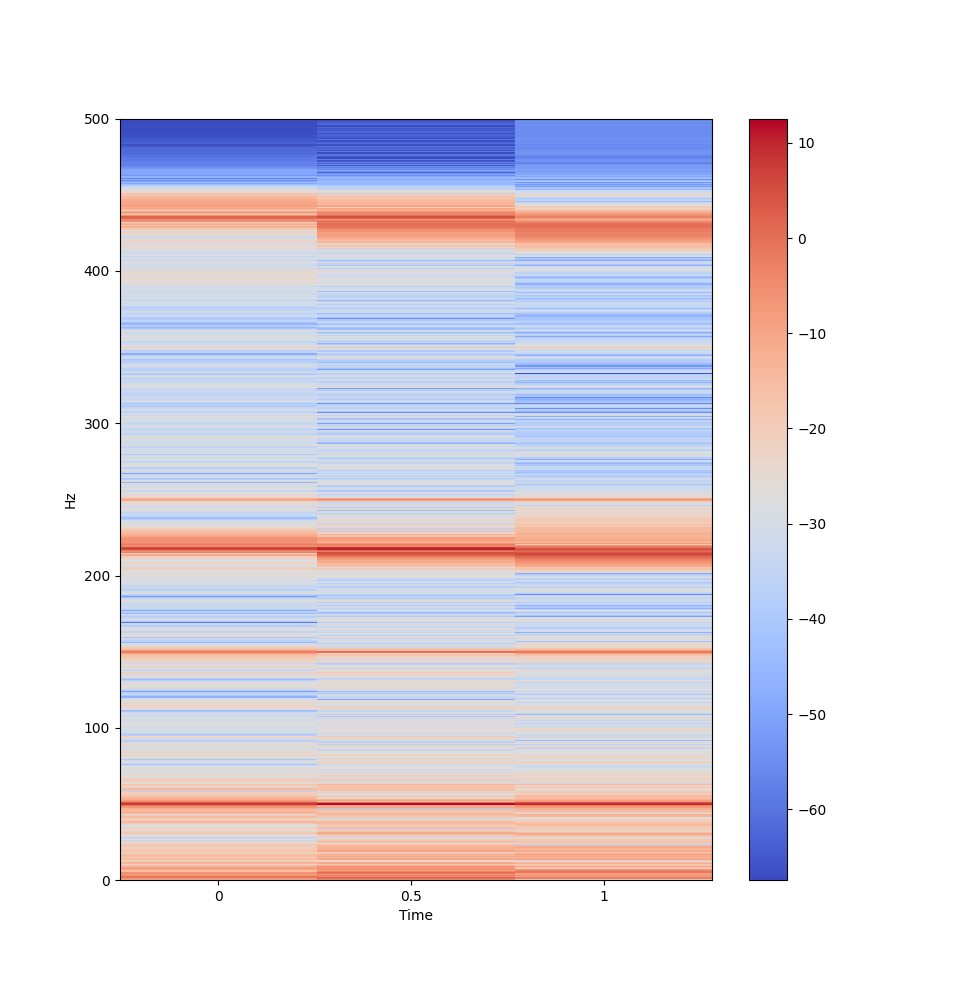
\includegraphics[width=0.6\textwidth]{przed-kompresja}
\caption{Spektrogram przed kompresją}
\end{figure}

\begin{figure}[h!]
\centering
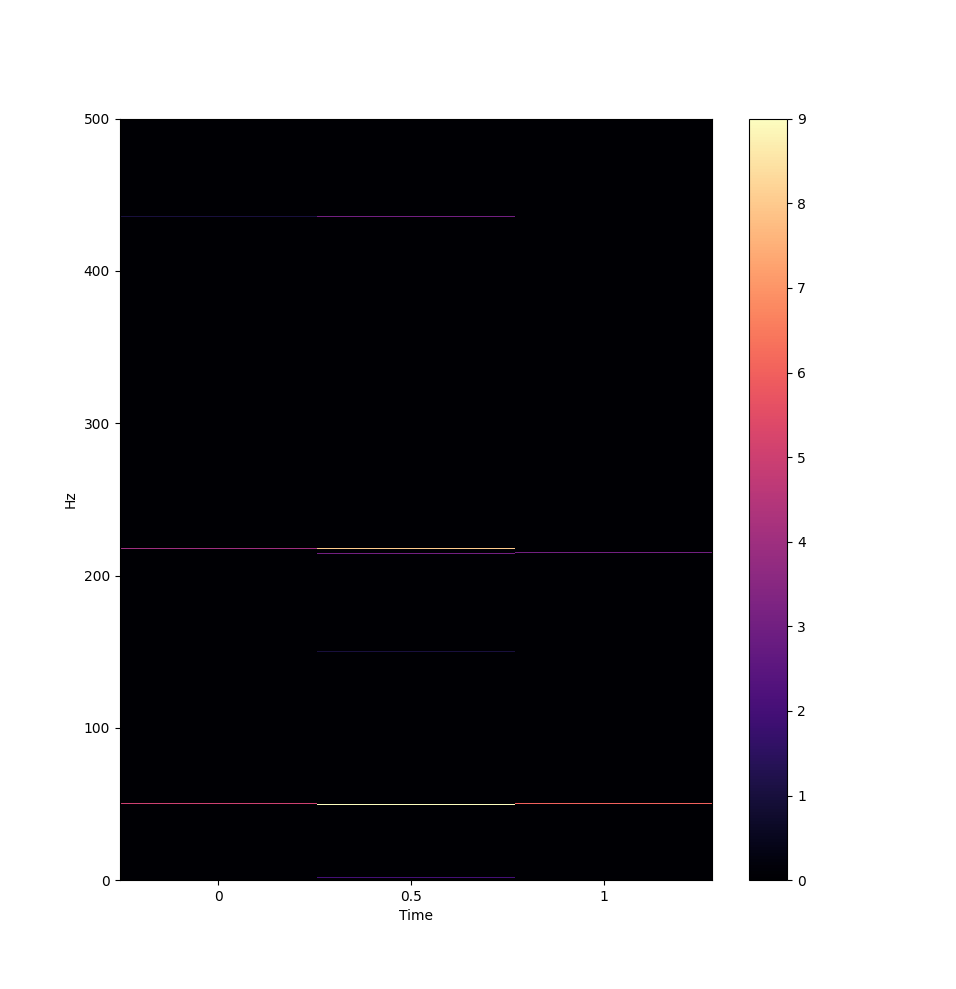
\includegraphics[width=0.6\textwidth]{po-kompresji}
\caption{Spektrogram po kompresji}
\end{figure}

\clearpage

\addcontentsline{toc}{section}{Dobieranie odpowiednich parametrów}
\section*{Dobieranie odpowiednich parametrów}

Parametry użyte w algorytmie (deno, freqdiff, freqmin) nie mają żadnego odzwierciedlenia matematycznego. Zostały dopasowane w ten sam sposób jaki działa sieć neuronowa algorytmów opartych o naukę maszynową - metoda prób i błędów. Stworzyłem pewnego rodzaju własną sieć neuronową, bardzo minimalistyczną, gdyż składa się tylko z 3 parametrów. Następnie na 8 poniżej przeanalizowanych próbkach dobrałem parametry tak, aby wyniki były jak najbardziej zadowalające.

\addcontentsline{toc}{section}{Jakość działania algorytmu}
\section*{Jakość działania algorytmu}

Dokładne porównanie z innymi algorytmami zostało przeanalizowane w jednej z kolejnych sekcji. Tutaj przeprowadzę dogłębną analizę kilku nagrań i rezultatów zwróconych wartości częstotliwości.

\clearpage

\addcontentsline{toc}{section}{Pierwsza próbka}
\section*{Pierwsza próbka}

\begin{figure}[h!]
\centering
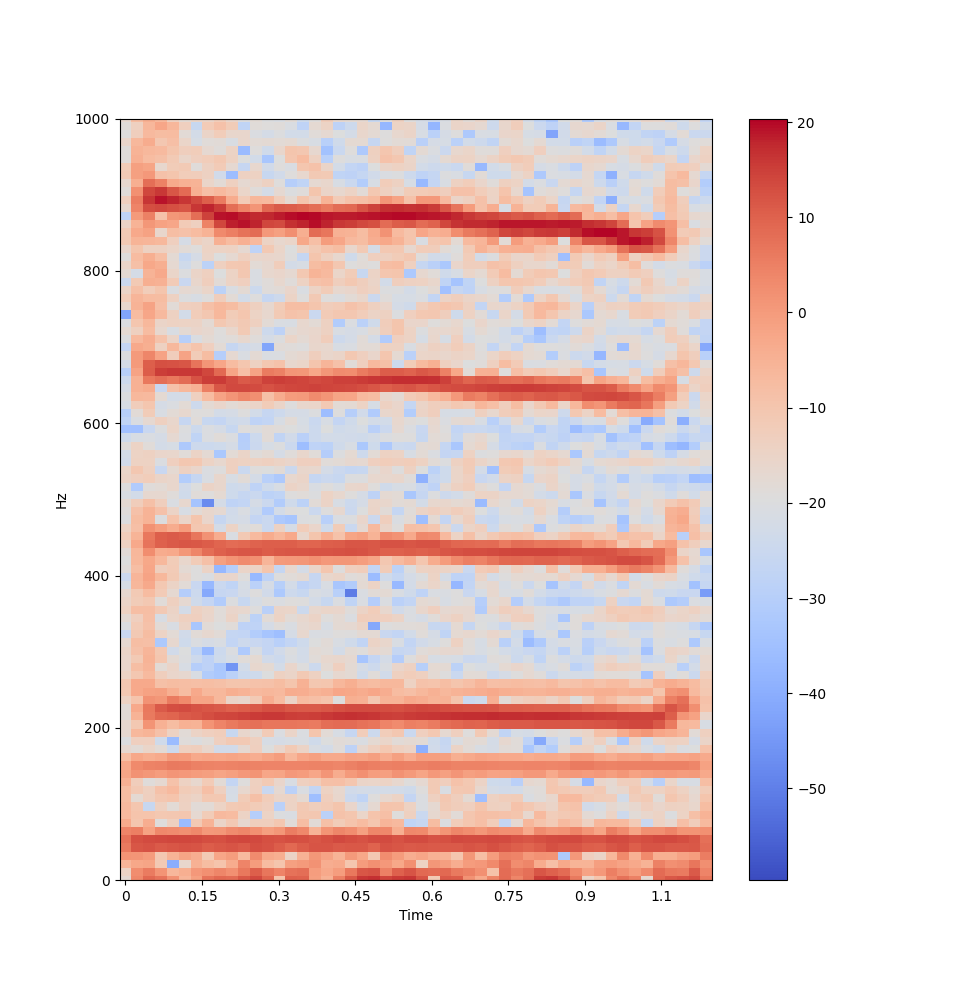
\includegraphics[width=0.9\textwidth]{female-audacity-normal-100}
\caption{Spektrogram nagrania female-audacity-normal-100.wav}
\end{figure}

\noindent Widełki: 200-225 Hz

\noindent Algorytm: 222.07 Hz\\

\noindent Algorytm poradził sobie w tym przypadku zaskakująco dobrze. Na spektrogramie widać wyraźnie artefakt w postaci poziomej linii na około 40 Hz. Jest on na tyle mocny, że prosto go pomylić z pierwszą harmoniczną, nawet mniej doświadczonemu człowiekowi. Dalej występuje już lżejszy artefakt w okolicach 180 Hz. Poprawnymi wartościami są częstotliwości trochę powyżej 200 Hz.

\clearpage

\addcontentsline{toc}{section}{Druga próbka}
\section*{Druga próbka}

\begin{figure}[h!]
\centering
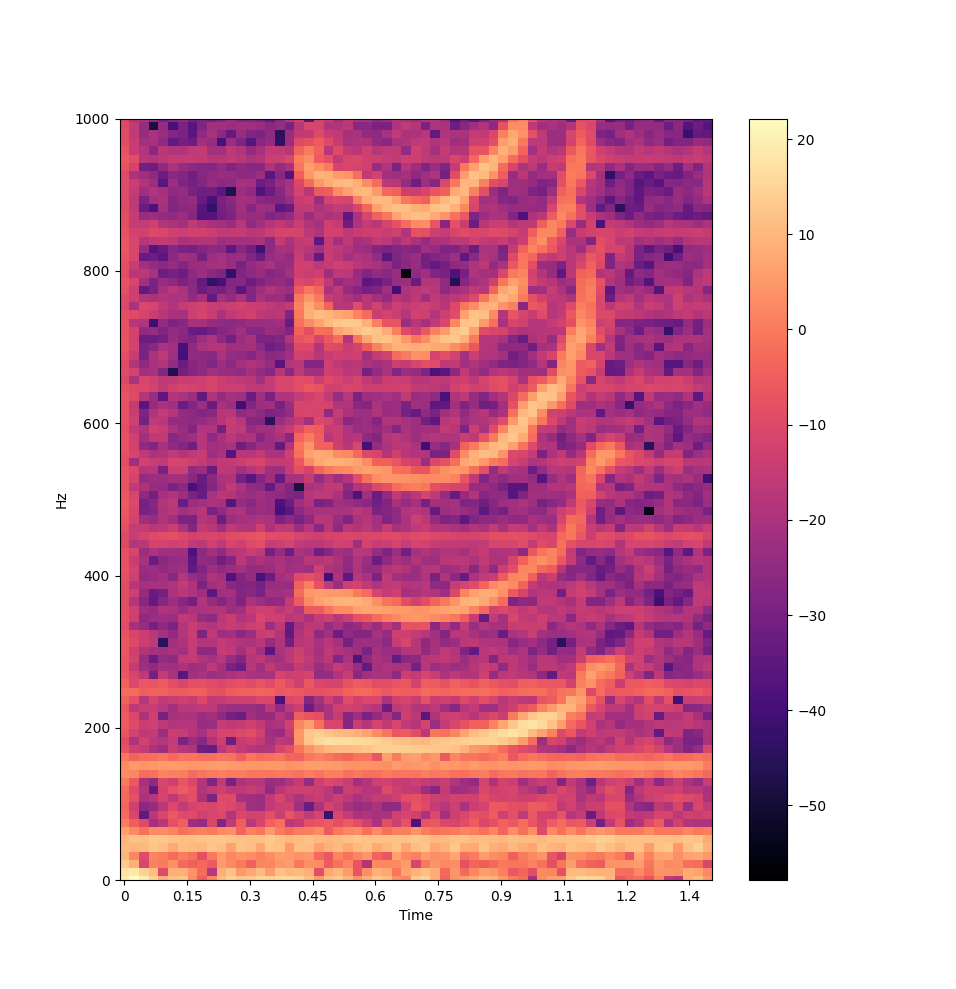
\includegraphics[width=0.9\textwidth]{female-audacity-normal-103}
\caption{Spektrogram nagrania female-audacity-normal-103.wav}
\end{figure}

\noindent Widełki: 160-190 Hz

\noindent Algorytm: 187.00 Hz\\

\noindent Kolejny trudny do analizy plik dźwiękowy. Tutaj w sposób okresowy występują poziome artefakty, najsilniejszy na około 30 Hz. Następny jest w okolicach 180 Hz i bardzo dobrze symuluje pierwszą harmoniczną. Dzięki zakrzywieniu spektrogramu człowiekowi prosto jest wydobyć prawdziwy głos z nagrania.

\clearpage

\addcontentsline{toc}{section}{Trzecia próbka}
\section*{Trzecia próbka}

\begin{figure}[h!]
\centering
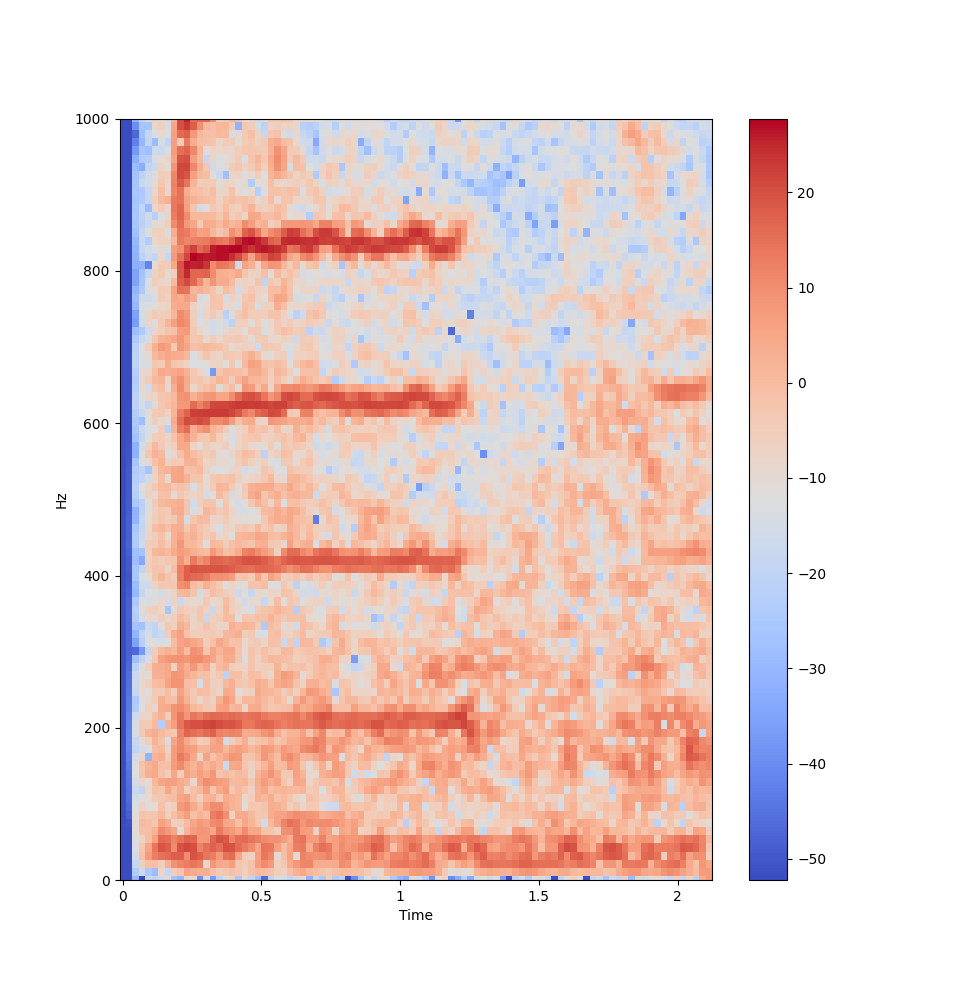
\includegraphics[width=0.9\textwidth]{female-iphone-normal-102}
\caption{Spektrogram nagrania female-iphone-normal-102.wav}
\end{figure}

\noindent Widełki: 200-220 Hz

\noindent Algorytm: 213.96 Hz\\

\noindent Nagranie niewyraźne, pomiędzy kolejnymi harmonicznymi występują szmery. Poziomy pasek na dolnych częstotliwościach może stawiać spore opory algorytmom odczytującym częstotliwość głosu. Dzięki zastosowaniu zmiany przedziału i osłabieniu głośności całego nagrania za pomocą algorytmu użytego w kompresji, algorytm odczytujący częstotliwość nie dał się zmylić i z perfekcyjną dokładnością ocenił nagranie.

\clearpage

\addcontentsline{toc}{section}{Czwarta próbka}
\section*{Czwarta próbka}

\begin{figure}[h!]
\centering
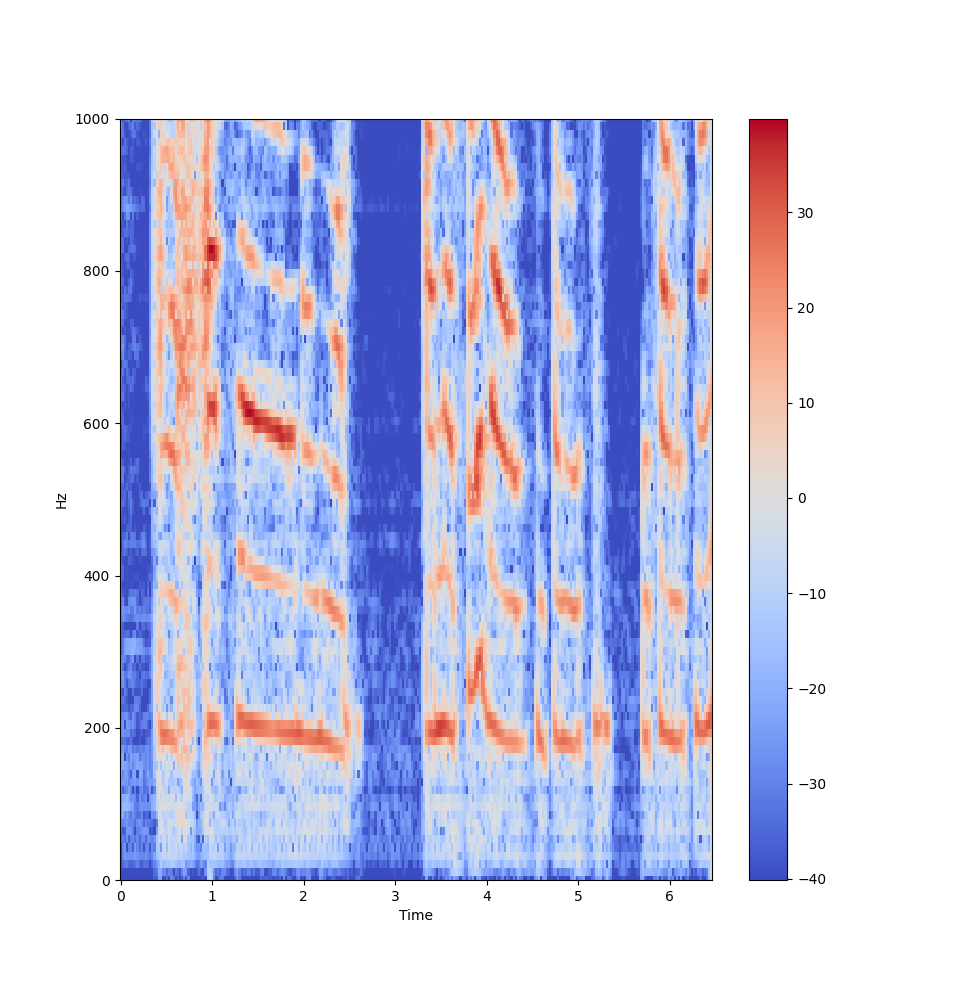
\includegraphics[width=0.9\textwidth]{female-twitch-normal-1}
\caption{Spektrogram nagrania female-twitch-normal-1.wav}
\end{figure}

\noindent Widełki: 180-200 Hz

\noindent Algorytm: 199.59 Hz\\

\noindent Algorytm zmieścił się na granicy błędu. Po spektrogramie widać, jak trudne było do analizy te nagranie. Brak ciągłości dźwięku, dziwne wariacje w okolicach 4 sekundy oraz przerwy. Uproszczeniem interpretacji jest brak artefaktów w postaci poziomych linii.

\clearpage

\addcontentsline{toc}{section}{Piąta próbka}
\section*{Piąta próbka}

\begin{figure}[h!]
\centering
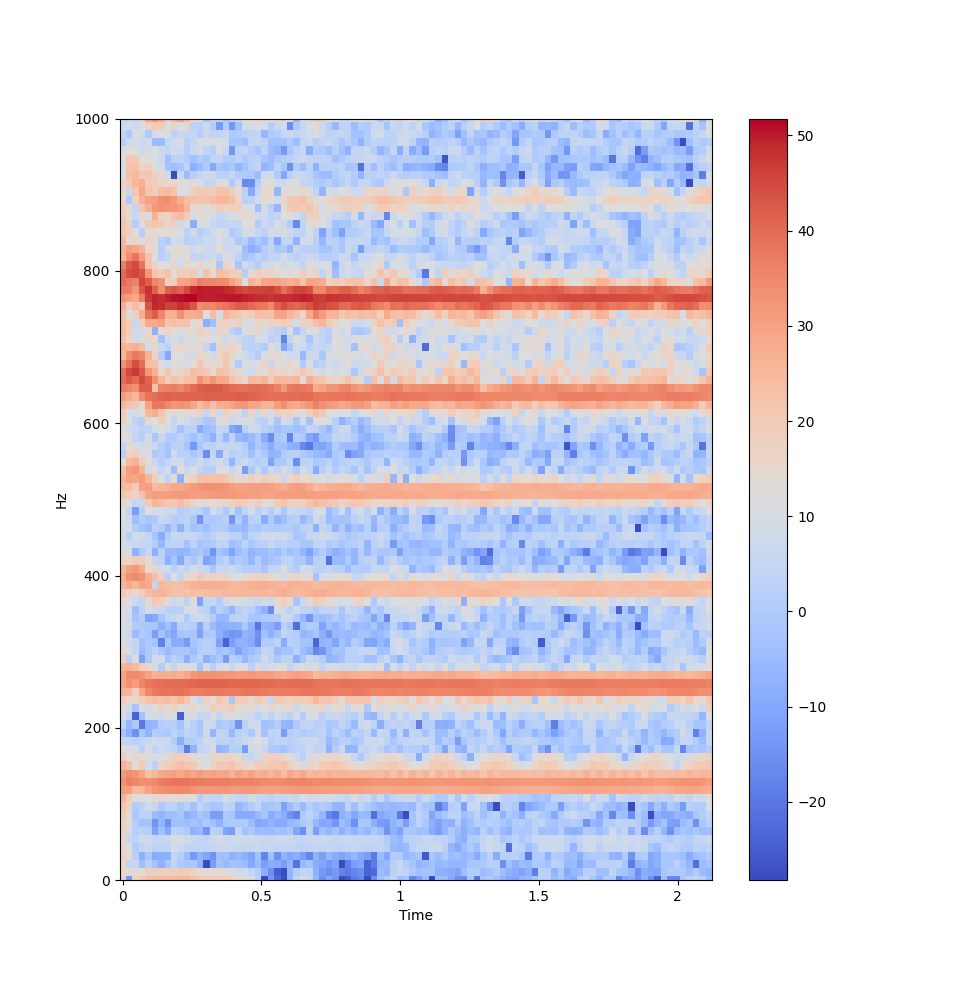
\includegraphics[width=0.9\textwidth]{male-discord-normal-2}
\caption{Spektrogram nagrania male-discord-normal-2.wav}
\end{figure}

\noindent Widełki: 115-135 Hz

\noindent Algorytm: 130.59 Hz\\

\noindent Ta próbka jest dość oczywista do analizy. Jedynym problematycznym miejscem są częstotliwości bliskiego 0 Hz dla czasu od 0 do 0.5 sekundy.

\clearpage

\addcontentsline{toc}{section}{Szósta próbka}
\section*{Szósta próbka}

\begin{figure}[h!]
\centering
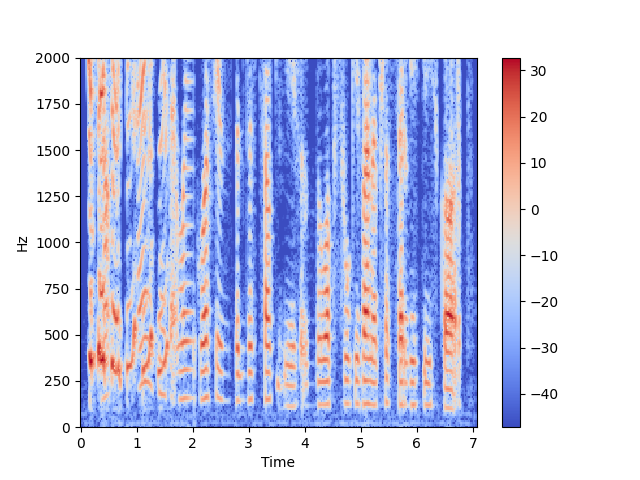
\includegraphics[width=0.9\textwidth]{male-discord-normal-102}
\caption{Spektrogram nagrania male-discord-normal-102.wav}
\end{figure}

\noindent Widełki: 110-140 Hz

\noindent Algorytm: 314.75 Hz\\

\noindent W tej próbce algorytm sobie teoretycznie nie poradził. Jednak sam nie jestem w stanie z pewnością stwierdzić jaką częstotliwość głosu miał autor nagrania. Widełki mieszczą się między 110-140 Hz, jednak na początku nagrania słychać śmiejącą się kobietę. Zakłóciła ona całość analizy znacznie zwiększając wartość rezultatu. Pokazuje to, że algorytm nie obsługuje wielu osób mówiących w jednym nagraniu.

\clearpage

\addcontentsline{toc}{section}{Siódma próbka}
\section*{Siódma próbka}

\begin{figure}[h!]
\centering
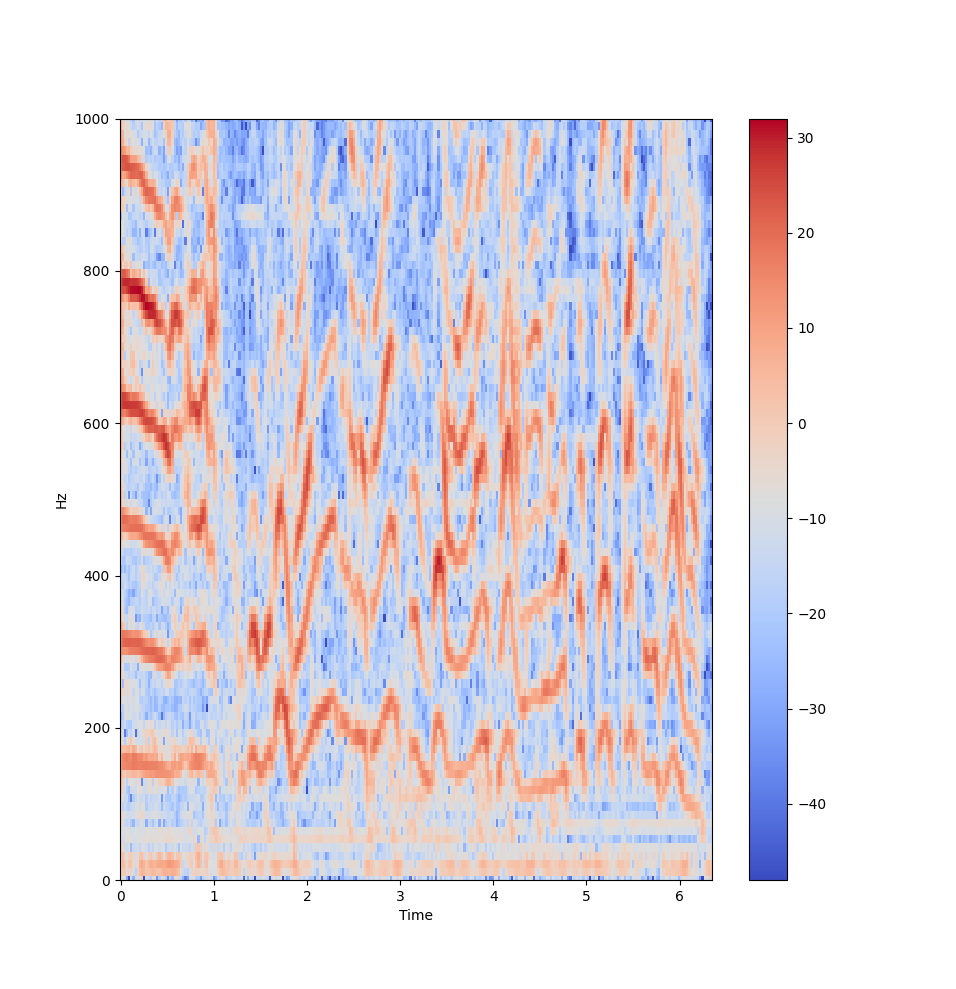
\includegraphics[width=0.9\textwidth]{male-twitch-normal-0}
\caption{Spektrogram nagrania male-twitch-normal-0.wav}
\end{figure}

\noindent Widełki: 140-165 Hz

\noindent Algorytm: 160.25 Hz\\

\noindent Kolejna problematyczna próbka, której spektrogram stanowią pokrętne linie. Występują artefakty na dolnych częstotliwościach, jednak są na tyle słabe, że algorytm je usuwający poradził sobie bez żadnego problemu.

\clearpage

\addcontentsline{toc}{section}{Ósma próbka}
\section*{Ósma próbka}

\begin{figure}[h!]
\centering
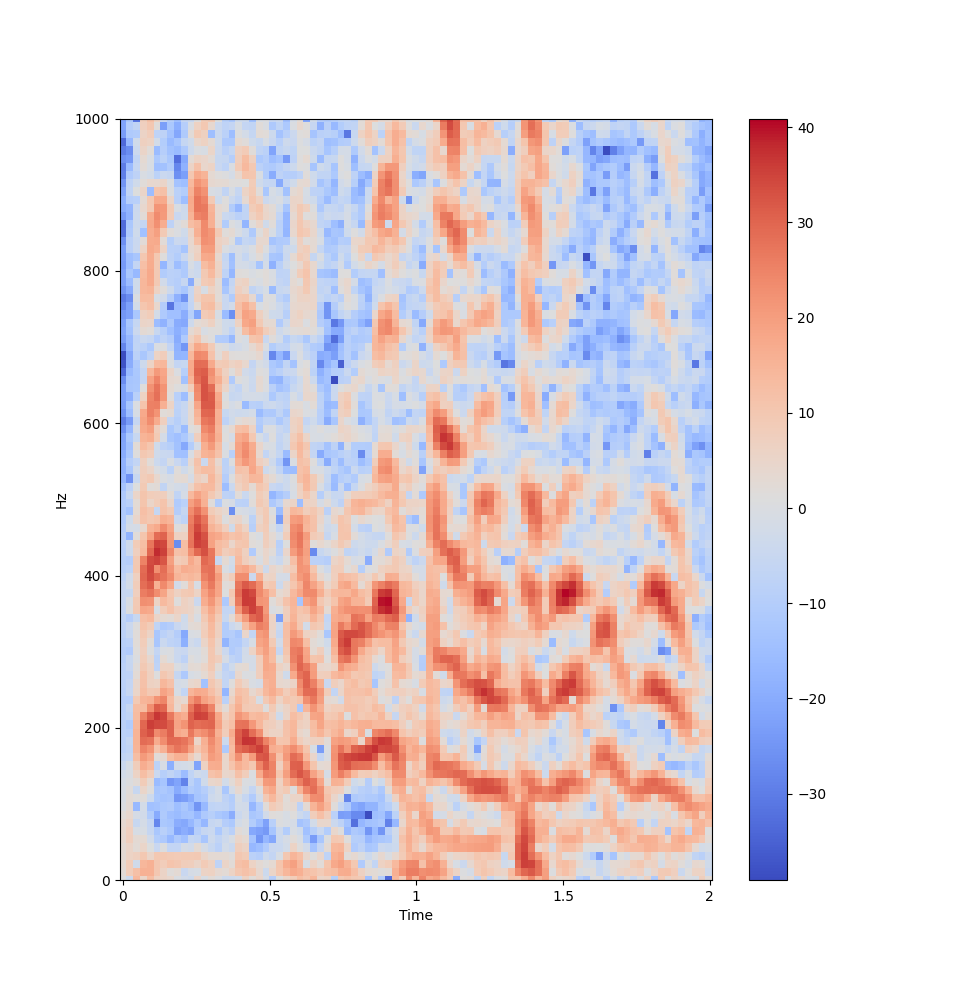
\includegraphics[width=0.9\textwidth]{male-youtube-normal-0}
\caption{Spektrogram nagrania male-youtube-normal-0.wav}
\end{figure}

\noindent Widełki: 150-190 Hz

\noindent Algorytm: 100.00 Hz\\

\noindent Drugie z ośmiu nagrań, które algorytm niepoprawnie określił. Problemem nie do pokonania dla mojego algorytmu była pionowa linia w okolicy 1.5 sekundy. Taki artefakt jest niezwykle zaskakujący i nietypowy. Został opisany w pierwszym raporcie \cite{report1}.

\clearpage

\addcontentsline{toc}{section}{Podsumowanie algorytmu}
\section*{Podsumowanie algorytmu}

Algorytm poradził sobie w 6 z 8 przypadków. W pierwszym przypadku poległ na analizy nagrania, gdzie mówi więcej, niż jedna osoba. Nie został do takiej analizy przystosowany, więc nie można wymagać, aby obsługiwał taki przypadek. W naszym projekcie w danym nagraniu mówi tylko jedna osoba z możliwymi zakłóceniami, w tym innymi osobami mówiącymi w tle. Druga próbka została źle przeanalizowana, gdyż budowa samego algorytmu nie pozwala na obsługę takich artefaktów. W takich przypadkach należałoby, użyć innego sposobu określenia częstotliwości. Możliwe, że pozostałe algorytmy poradziły sobie w tej próbce lepiej.


\clearpage

\section{Znajdowanie pierwszej harmonicznej}
\label{sec:harmonic}

Mój algorytm wywodzi się bezpośrednio z definicji informacji dla naszego projektu. Za kluczową uznajemy pierwszą harmoniczną głosu, dlatego właśnie na tym skupiłem się tworząc go.
       
\addcontentsline{toc}{section}{Sposób działania}
\section*{Sposób działania}

\noindent Cały algorytm podzielony jest na kilka funkcji. Główną jego częścią jest funkcja "first-harmonics" iterująca po całej dwuwymiarowej tablicy wyników STFT, która reprezentuje głośność poszczególnych częstotliwość w danej chwili nagrania. Przede wszystkim szuka lokalnych maksimów dla danej chwili, gdzie głośność przekracza pewien próg (więcej o nim w podsekcji "Dobór parametrów").\\

\noindent Następnie korzystając z krótkiej funkcji "check-if-harmonic" sprawdza czy znaleziona przez nią częstotliwość jest jedną z harmonicznych głosu ludzkiego, czy jedynie zakłóceniem. Dokonuje tego poprzez analizę wyższych częstotliwości szukając kolejnych harmonicznych z pewną tolerancją.\\

\noindent Pierwsza znalezioną w powyższy sposób harmoniczna (zaczynając szukanie od najniższych częstotliwości) zostaje dopisana do tablicy wyników. W ten sposób powstaje lista częstotliwości pierwszej harmonicznej względem czasu. Tę listę następnie filtruję za pomocą funkcji "values-in-range" usuwając częstotliwości poniżej 60 lub powyżej 500 Hz. Pozbywam się w ten sposób momentów cichych oraz większość wyników, które powstały w skutek pomyłki algorytmu (w zależności od zakłóceń w nagraniu może to być nawet połowa wszystkich niezerowych wyników).

\newpage
       
\addcontentsline{toc}{section}{Dobór parametrów}
\section*{Dobór parametrów}

\noindent Wszystkie parametry zostały dobrane wedle zasady prób i błędów, dlatego mogą nie być one optymalne. Dawały jednak zadowalające wyniki dla próbek testowych.\\

\noindent Próg głośności jest używany zarówno podczas szukania maksimów lokalnych częstotliwości jako prosty filtr, jak i później podczas szukania kolejnych harmonicznych by sprawdzić czy znalezione maksimum jest jedną z nich. Obecna jego wartość wynosi połowę maksymalnej głośności dla danego momentu w czasie w decybelach. Oryginalnie używałem jednej wartości dla całego nagrania, jednak w ten sposób sprawdza się on lepiej w przypadku nagrań  o cichszych i głośniejszych momentach.\\

\noindent Głębokość sprawdzania określa ile kolejnych harmonicznych trzeba znaleźć by uznać analizowaną częstotliwość za harmoniczną. Obecnie wartość ta wynosi 5 i jest to jeden z najcięższych do właściwego dobrania parametrów.\\

\noindent Niedokładność sprawdzania to promień przedziału w jakim poszukiwana jest kolejna harmoniczna, która w teorii powinna być wielokrotnością częstotliwości pierwszej harmonicznej. W praktyce ze względu na charakter ludzkiego głosu oraz STFT są małe odstępstwa. Obecnie wartość ta wynosi 3, co oznacza +/- 3 przedziały częstotliwości jakie daje STFT.\\

\noindent Minimum i maksimum akceptowalnych wyników wynoszą odpowiednio 60 i 500 Hz tak by z całą pewnością nie zostały usunięte sensowne wyniki dla pierwszej harmonicznej głosu.

\newpage

\addcontentsline{toc}{section}{Pierwsza próbka}
\section*{Pierwsza próbka}

\begin{figure}[h!]
\centering
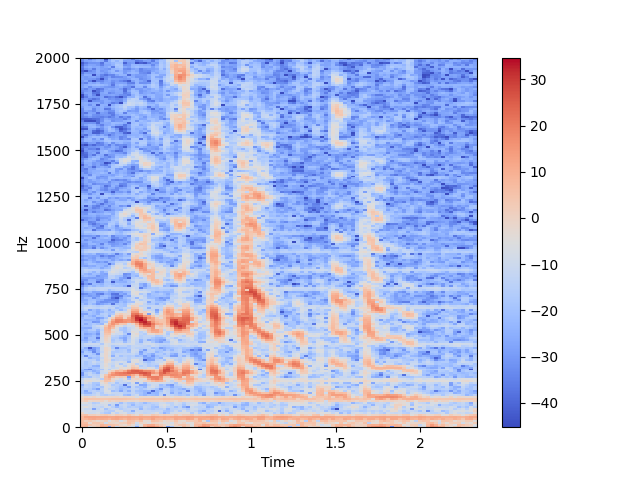
\includegraphics[width=0.9\textwidth]{wykresy/pochmara-patryk/female-audacity-normal-102.png}
\caption{Spektrogram nagrania female-audacity-normal-102.wav}
\end{figure}

\noindent Widełki: 150-350 Hz

\noindent Algorytm: 174 Hz\\

\noindent Ciekawa próbka z dużą wariacją, średnia  z wartości pierwszej harmonicznej w całym nagraniu poprawie trafia do pożądanego przedziału pomimo artefaktu około 50 Hz.

\newpage

\addcontentsline{toc}{section}{Druga próbka}
\section*{Druga próbka}

\begin{figure}[h!]
\centering
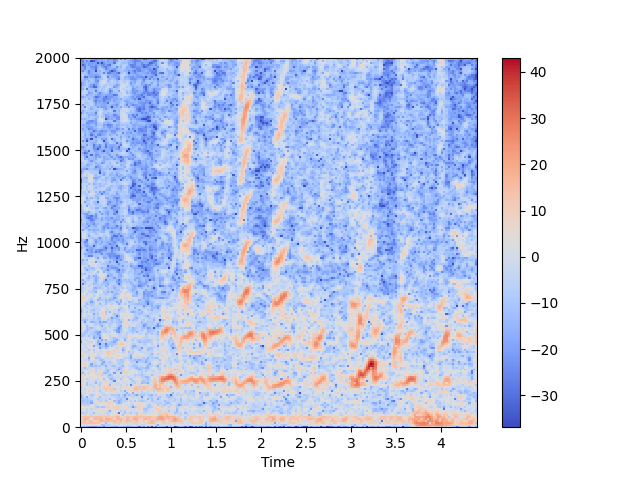
\includegraphics[width=0.9\textwidth]{wykresy/pochmara-patryk/female-iphone-normal-103.png}
\caption{Spektrogram nagrania female-iphone-normal-103.wav}
\end{figure}

\noindent Widełki: 200-310 Hz

\noindent Algorytm: 236 Hz\\

\noindent Ponownie poprawny wynik, mimo szumów na niskich częstotliwościach. Fakt, że stosunkowo duża część nagrania nie zawiera głosu nie przeszkadza algorytmowi.

\newpage

\addcontentsline{toc}{section}{Trzecia próbka}
\section*{Trzecia próbka}

\begin{figure}[h!]
\centering
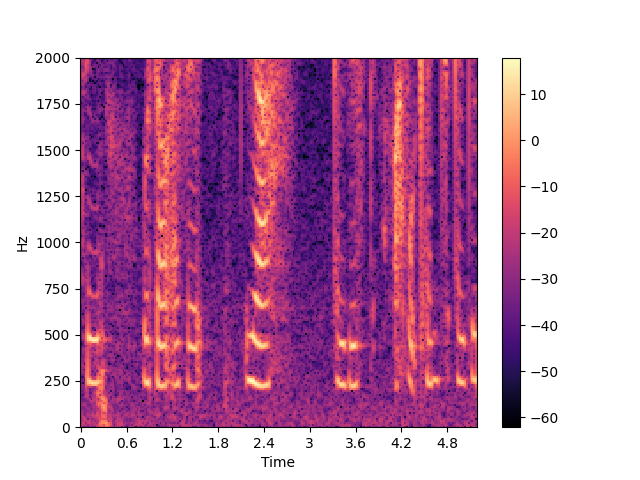
\includegraphics[width=0.9\textwidth]{wykresy/pochmara-patryk/female-twitch-normal-0.png}
\caption{Spektrogram nagrania female-twitch-normal-0.wav}
\end{figure}

\noindent Widełki: 200-240 Hz

\noindent Algorytm: 225 Hz\\

\noindent Nagranie z serwisu Twitch, widocznie cichsze od pozostałych (skala decybeli po prawej) także nie sprawia problemów.

\newpage

\addcontentsline{toc}{section}{Czwarta próbka}
\section*{Czwarta próbka}

\begin{figure}[h!]
\centering
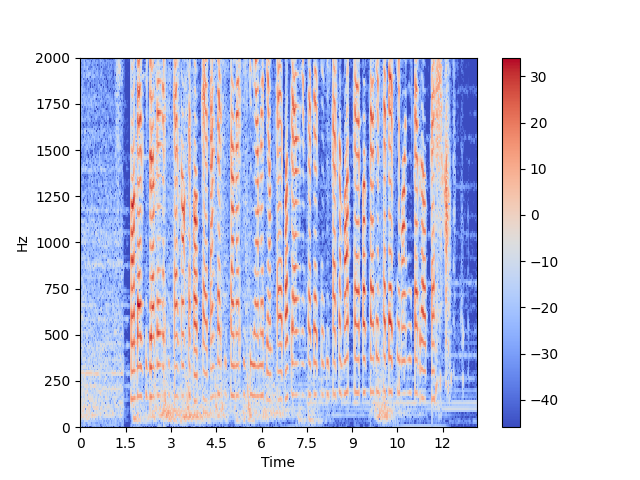
\includegraphics[width=0.9\textwidth]{wykresy/pochmara-patryk/male-discord-normal-101.png}
\caption{Spektrogram nagrania male-discord-normal-101.wav}
\end{figure}

\noindent Widełki: 135-180 Hz

\noindent Algorytm: 257 Hz\\

\noindent Wyraźna porażka, chociaż nie tyle samego algorytmu ile jego parametrów. Pierwsza harmoniczna na nagraniu jest zbyt cicha by przekroczyć próg głośności, jednak gdyby został obniżony wyniki dla innych nagrań (szczególnie tych z szumami) utraciłyby dokładność.

\newpage

\addcontentsline{toc}{section}{Piąta próbka}
\section*{Piąta próbka}

\begin{figure}[h!]
\centering
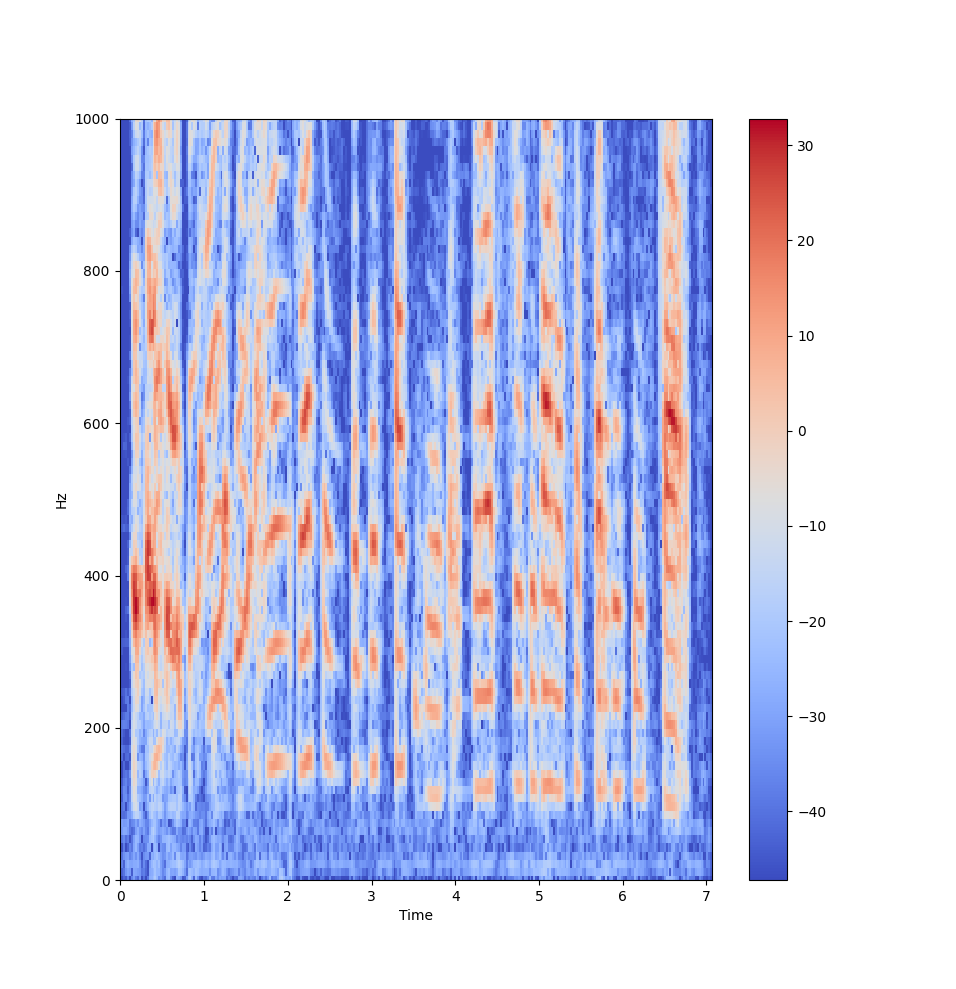
\includegraphics[width=0.9\textwidth]{wykresy/pochmara-patryk/male-discord-normal-102.png}
\caption{Spektrogram nagrania male-discord-normal-102.wav}
\end{figure}

\noindent Widełki: 120-170 Hz

\noindent Algorytm: 193 Hz\\

\noindent To nagranie jest bardzo trudne do sklasyfikowania, ponieważ na początku słychać śmiech kobiety, a nagranie zawiera głos mężczyzny. Wyraźnie wpłynęło to na wynik algorytmu. Nie jest to bardzo duże odchylenie, ale wystarczające by uniemożliwić proste określenie płci mówiącego.

\newpage

\addcontentsline{toc}{section}{Szósta próbka}
\section*{Szósta próbka}

\begin{figure}[h!]
\centering
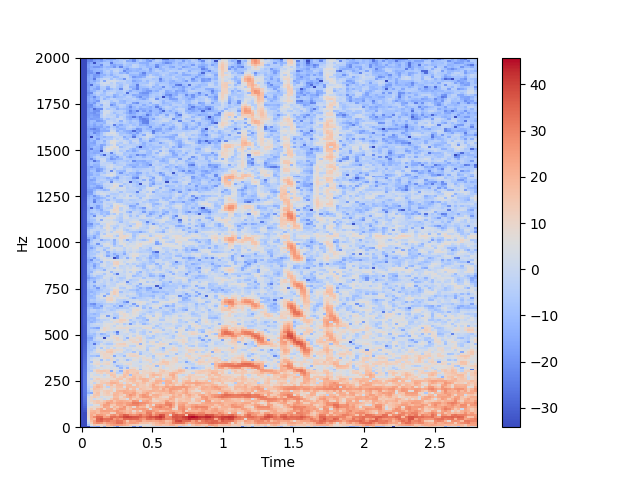
\includegraphics[width=0.9\textwidth]{wykresy/pochmara-patryk/male-iphone-normal-100.png}
\caption{Spektrogram nagrania male-iphone-normal-100.wav}
\end{figure}

\noindent Widełki: 160-190 Hz

\noindent Algorytm: 64 Hz\\

\noindent Bardzo silne szumy, w dodatku rozciągnięte na cały przedział 60-250 Hz skutecznie uniemożliwiły poprawną analizę poprzez algorytm. Chociaż prawdopodobnie zwiększenie parametru głębokości sprawdzania mogłoby pozwolić na uzyskanie lepszych rezultatów w tym wypadku.

\newpage

\addcontentsline{toc}{section}{Siódma próbka}
\section*{Siódma próbka}

\begin{figure}[h!]
\centering
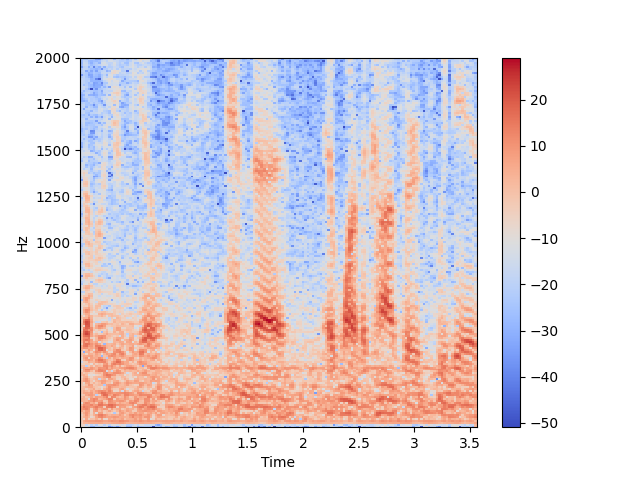
\includegraphics[width=0.9\textwidth]{wykresy/pochmara-patryk/male-youtube-normal-4.png}
\caption{Spektrogram nagrania male-youtube-normal-4.wav}
\end{figure}

\noindent Widełki: 55-80 Hz

\noindent Algorytm: 93 Hz\\

\noindent Kolejne trudne nagranie, zwłaszcza, że głos mężczyzny na nim mówiącego jest bardzo niski i trudno rozróżnić go od szumów. Za ciekawy uważam fakt, że o ile algorytm podał za wysoką wartość, to jest ona bliska pożądanej, a co więcej w zupełności wystarczająca by poprawnie sklasyfikować głos jako męski.

\clearpage

\section{Porównanie algorytmów}
\label{sec:compare}

\addcontentsline{toc}{section}{Tabela wyników}
\section*{Tabela wyników}

\begin{center}
\resizebox{\textwidth}{!}{
\begin{tabular}{ |c|c|c|c|c|c|c|c|c| } 
 \hline
Nazwa pliku & Dolna granica [Hz] & Górna granica [Hz] & R Wartość & R Poprawny & R Odchylenie & P Wartość & P Poprawny & P Odchylenie \\
 \hline
female-audacity-high-100 & 267 & 314 & 305 & Prawda & 0\% & 301 & Prawda & 0\% \\
female-audacity-high-101 & 463 & 582 & 500 & Prawda & 0\% & 495 & Prawda & 0\% \\
female-audacity-high-102 & 440 & 550 & 500 & Prawda & 0\% & 0 & Flasz & 100\% \\
female-audacity-high-103 & 330 & 522 & 500 & Prawda & 0\% & 462 & Prawda & 0\% \\
female-audacity-low-100 & 185 & 205 & 200 & Prawda & 0\% & 193 & Prawda & 0\% \\
female-audacity-low-101 & 190 & 220 & 210 & Prawda & 0\% & 204 & Prawda & 0\% \\
female-audacity-low-102 & 155 & 270 & 500 & Flasz & 85\% & 172 & Prawda & 0\% \\
female-audacity-normal-100 & 210 & 230 & 222 & Prawda & 0\% & 215 & Prawda & 0\% \\
female-audacity-normal-101 & 195 & 220 & 214 & Prawda & 0\% & 204 & Prawda & 0\% \\
female-audacity-normal-102 & 150 & 350 & 305 & Prawda & 0\% & 172 & Prawda & 0\% \\
female-audacity-normal-103 & 170 & 270 & 187 & Prawda & 0\% & 183 & Prawda & 0\% \\
female-audacity-normal-104 & 110 & 170 & 126 & Prawda & 0\% & 129 & Prawda & 0\% \\
female-discord-high-100 & 190 & 370 & 191 & Prawda & 0\% & 0 & Flasz & 100\% \\
female-discord-low-100 & 170 & 340 & 205 & Prawda & 0\% & 204 & Prawda & 0\% \\
female-discord-normal-100 & 160 & 290 & 195 & Prawda & 0\% & 183 & Prawda & 0\% \\
female-iphone-high-100 & 380 & 470 & 98 & Flasz & 74\% & 419 & Prawda & 0\% \\
female-iphone-high-101 & 380 & 570 & 405 & Prawda & 0\% & 387 & Prawda & 0\% \\
female-iphone-high-102 & 540 & 615 & 500 & Flasz & 7\% & 441 & Flasz & 18\% \\
female-iphone-low-100 & 190 & 245 & 223 & Prawda & 0\% & 215 & Prawda & 0\% \\
female-iphone-low-101 & 170 & 205 & 195 & Prawda & 0\% & 193 & Prawda & 0\% \\
female-iphone-normal-100 & 215 & 240 & 226 & Prawda & 0\% & 215 & Prawda & 0\% \\
female-iphone-normal-101 & 200 & 250 & 242 & Prawda & 0\% & 236 & Prawda & 0\% \\
female-iphone-normal-102 & 195 & 220 & 213 & Prawda & 0\% & 204 & Prawda & 0\% \\
female-iphone-normal-103 & 200 & 310 & 258 & Prawda & 0\% & 231 & Prawda & 0\% \\
female-iphone-normal-104 & 230 & 320 & 139 & Flasz & 39\% & 312 & Prawda & 0\% \\
female-twitch-normal-0 & 200 & 240 & 76 & Flasz & 62\% & 226 & Prawda & 0\% \\
female-twitch-normal-1 & 180 & 220 & 199 & Prawda & 0\% & 193 & Prawda & 0\% \\
male-audacity-normal-100 & 100 & 140 & 124 & Prawda & 0\% & 118 & Prawda & 0\% \\
male-discord-high-0 & 360 & 390 & 379 & Prawda & 0\% & 366 & Prawda & 0\% \\
male-discord-high-1 & 485 & 525 & 500 & Prawda & 0\% & 0 & Flasz & 100\% \\
male-discord-high-2 & 365 & 405 & 374 & Prawda & 0\% & 387 & Prawda & 0\% \\
male-discord-high-3 & 305 & 385 & 345 & Prawda & 0\% & 322 & Prawda & 0\% \\
male-discord-low-0 & 85 & 105 & 98 & Prawda & 0\% & 193 & Flasz & 83\% \\
male-discord-low-1 & 100 & 115 & 133 & Flasz & 15\% & 118 & Flasz & 2\% \\
male-discord-low-100 & 120 & 150 & 134 & Prawda & 0\% & 129 & Prawda & 0\% \\
male-discord-low-2 & 70 & 110 & 101 & Prawda & 0\% & 96 & Prawda & 0\% \\
male-discord-low-3 & 85 & 100 & 100 & Prawda & 0\% & 96 & Prawda & 0\% \\
male-discord-normal-0 & 90 & 120 & 103 & Prawda & 0\% & 96 & Prawda & 0\% \\
male-discord-normal-1 & 105 & 130 & 122 & Prawda & 0\% & 118 & Prawda & 0\% \\
male-discord-normal-101 & 135 & 180 & 172 & Prawda & 0\% & 172 & Prawda & 0\% \\
male-discord-normal-102 & 120 & 300 & 250 & Prawda & 0\% & 129 & Prawda & 0\% \\
male-discord-normal-103 & 130 & 155 & 144 & Prawda & 0\% & 279 & Flasz & 80\% \\
male-discord-normal-2 & 115 & 150 & 130 & Prawda & 0\% & 129 & Prawda & 0\% \\
male-discord-normal-3 & 80 & 140 & 104 & Prawda & 0\% & 96 & Prawda & 0\% \\
male-discord-normal-4 & 75 & 120 & 101 & Prawda & 0\% & 96 & Prawda & 0\% \\
male-iphone-normal-100 & 160 & 190 & 145 & Flasz & 9\% & 64 & Flasz & 60\% \\
male-iphone-normal-101 & 115 & 150 & 122 & Prawda & 0\% & 96 & Flasz & 16\% \\
male-twitch-normal-0 & 115 & 235 & 160 & Prawda & 0\% & 150 & Prawda & 0\% \\
male-youtube-normal-0 & 90 & 230 & 100 & Prawda & 0\% & 150 & Prawda & 0\% \\
male-youtube-normal-4 & 55 & 80 & 75 & Prawda & 0\% & 129 & Flasz & 61\% \\
 \hline
\end{tabular}}
\end{center}

\clearpage

\addcontentsline{toc}{section}{Ocena algorytmów}
\section*{Ocena algorytmów}

W powyższej tabeli widać jak nasze algorytmy (oznaczone odpowiednio R i P) sprawdziły się dla nagrań, które mamy w naszej bazie. Dla zdecydowanej większości nagrań zwróciły one poprawne wyniki. Na 50 próbek algorytm R sprawdził się w 42 przypadkach, a algorytm P w 40. Są tylko 2 pliki, dla których oba algorytmy zawiodły, jednak algorytm R był bliski poprawnego wyniku (poniżej 10\% pomyłki).
Algorytm P niestety czasami jest bardzo odległy od odpowiedzi, jednak w niektórych przypadkach radzi sobie lepiej od R. Są to rzadkie nagrania, gdzie występują głośne zakłócenia o konkretnej częstotliwości. Algorytm P dzięki analizie harmonicznych jest w stanie je zignorować, a R daje się im zmylić. Jednak w sytuacji, gdy zakłócenia są szumem rozpiętym na wielu częstotliwościach zazwyczaj lepszy jest R.
Podsumowując o ile P potrafi dobrze przeanalizować specyficzne nagrania, częściej dokładniejszy jest R. W dalszych etapach projektu oba algorytmy będą jeszcze ulepszane tak by ich współpraca pozwalała na jak najlepszą analizę głosu.

\clearpage

\printbibliography[title=Bibliografia]

\end{document}
